\documentclass[a4paper, 11pt]{article}\usepackage[]{graphicx}\usepackage[]{color}
%% maxwidth is the original width if it is less than linewidth
%% otherwise use linewidth (to make sure the graphics do not exceed the margin)
\makeatletter
\def\maxwidth{ %
  \ifdim\Gin@nat@width>\linewidth
    \linewidth
  \else
    \Gin@nat@width
  \fi
}
\makeatother

\definecolor{fgcolor}{rgb}{0.345, 0.345, 0.345}
\newcommand{\hlnum}[1]{\textcolor[rgb]{0.686,0.059,0.569}{#1}}%
\newcommand{\hlstr}[1]{\textcolor[rgb]{0.192,0.494,0.8}{#1}}%
\newcommand{\hlcom}[1]{\textcolor[rgb]{0.678,0.584,0.686}{\textit{#1}}}%
\newcommand{\hlopt}[1]{\textcolor[rgb]{0,0,0}{#1}}%
\newcommand{\hlstd}[1]{\textcolor[rgb]{0.345,0.345,0.345}{#1}}%
\newcommand{\hlkwa}[1]{\textcolor[rgb]{0.161,0.373,0.58}{\textbf{#1}}}%
\newcommand{\hlkwb}[1]{\textcolor[rgb]{0.69,0.353,0.396}{#1}}%
\newcommand{\hlkwc}[1]{\textcolor[rgb]{0.333,0.667,0.333}{#1}}%
\newcommand{\hlkwd}[1]{\textcolor[rgb]{0.737,0.353,0.396}{\textbf{#1}}}%

\usepackage{framed}
\makeatletter
\newenvironment{kframe}{%
 \def\at@end@of@kframe{}%
 \ifinner\ifhmode%
  \def\at@end@of@kframe{\end{minipage}}%
  \begin{minipage}{\columnwidth}%
 \fi\fi%
 \def\FrameCommand##1{\hskip\@totalleftmargin \hskip-\fboxsep
 \colorbox{shadecolor}{##1}\hskip-\fboxsep
     % There is no \\@totalrightmargin, so:
     \hskip-\linewidth \hskip-\@totalleftmargin \hskip\columnwidth}%
 \MakeFramed {\advance\hsize-\width
   \@totalleftmargin\z@ \linewidth\hsize
   \@setminipage}}%
 {\par\unskip\endMakeFramed%
 \at@end@of@kframe}
\makeatother

\definecolor{shadecolor}{rgb}{.97, .97, .97}
\definecolor{messagecolor}{rgb}{0, 0, 0}
\definecolor{warningcolor}{rgb}{1, 0, 1}
\definecolor{errorcolor}{rgb}{1, 0, 0}
\newenvironment{knitrout}{}{} % an empty environment to be redefined in TeX

\usepackage{alltt}
\usepackage[OT1]{fontenc}
\usepackage{url}

\usepackage{graphicx}
\usepackage{tikz}
\usetikzlibrary{decorations,arrows,shapes}
\usepackage[margin=0.9in]{geometry}
\usepackage{url}
\usepackage{hyperref}
\usepackage{listings}
\usepackage{xspace}
\usepackage[numbers]{natbib}
\bibliographystyle{plainnat}
\setlength{\parindent}{0mm}
\setlength{\parskip}{1mm}
\newcommand{\commentout}[1]{}
\newcommand{\al}{$\alpha$-level\xspace}
\newcommand{\eg}{\em e.g.}
\newcommand{\ie}{\em i.e.}
\newcommand{\gmcp}{\texttt{gMCP}\xspace}
\newcommand{\gact}{\texttt{gACT}\xspace}
\IfFileExists{upquote.sty}{\usepackage{upquote}}{}
\begin{document}

% \VignetteEngine{knitr::knitr}
% \VignetteIndexEntry{Graphical approaches for multiple endpoint problems using weighted parametric tests}

\title{Weighted parametric tests defined by graphs} 

\author{Florian Klinglmueller}

\maketitle

\tableofcontents


\section{Introduction}
\label{sec:intro}

This document describes how to use \gmcp to construct, conduct and evaluate
multiple comparison procedures based on  weighted parametric tests
which are defined by directed graphs. In addition to sequentially
rejective Bonferroni procedures \gmcp provides functionality to
construct tests that take advantage of (partial) knowledge of the
the joint distribution of the $p$-values associated with multiple
hypotheses. For the time being \gmcp implements the case of multiple
inferences based on one-sided $z$-tests. 

If the joint distribution of the p-values is known the sequentially
rejective tests described in \cite{bretzEtAl2009graphical} may be
performed using corresponding closed test procedures based on weighted
min-$p$ tests for each intersection hypotheses.  It is assumed that
under the global null hypothesis
$(\Phi^{-1}(1-p_1),\ldots,\Phi^{-1}(1-p_m))$ follow a multivariate
normal distribution with correlation matrix $\Sigma$ where
$\Phi^{-1}$ denotes the inverse of the standard normal
distribution function. For example, this is the case if $p_1,\ldots,
  p_m$ are the raw p-values from one-sided $z$-tests for each of the
elementary hypotheses where the correlation between z-test statistics
is generated by an overlap in the observations (e.g. comparison with a
common control, group-sequential analyses etc.). An application of the
transformation $\Phi^{-1}(1-p_i)$ to raw p-values from a two-sided
test will not in general lead to a multivariate normal
distribution. Partial knowledge of the correlation matrix is
supported.  If the correlation matrix of a given subset of test
statistics is known tests for intersection hypotheses containing the
associated elementary hypotheses are computed using the multivariate
distribution under the respective null. Hence, the consonance condition
necessary for the shortcut that yields sequentially rejective tests
can no longer be guaranteed using this approach. Hence, the whole
closed test is performed. For an exhaustive theoretical specification
of the general statistical principle please see \cite[Section
3.2]{Bretz11}.

As an example we will use graph based procedures introduced in
Example 1 and Example 2 of \cite[Sections 2 and 3.2]{Bretz11}. 

% \section{Statement of Problem}
% \label{sec:prob}

% Consider the problem of testing $m$ null hypotheses $H_1^0,...,H_m^0$
% at multiple significance level $\alpha$. Let $S_1,...,S_m$ denote the
% test statistics associated with the elementary
% hypotheses\footnote{Note that at this point we only consider test
%   normally distributed test statistics with known variance}.  The
% graphical approach \cite{paper1} provides a convenient tool to define
% weighted sequential tests that capture the contextual relationships
% between elementary hypotheses, \eg~the hypotheses might be of
% different importance in the sense that 
% rejecting a hypotheses of low importance while retaining one of higher
% importance might not be clinically relevant. This is done by defining
% initial weights specifying the proportion of the overall \al allocated
% to each elementary hyptheses. Weights for the elementary hypotheses of
% smaller intersection hypotheses are then recursively determined
% according to an \al reallocation scheme which is specified by means of
% a directed graph. Suppose that for some pairs of hypotheses pairwise
% correlations of the respective test statistics
% $\textrm{cor}(S_i,S_j)$ are known and let $C := (c_{ij})_{i,j
%   \in \{1,...,m\}}$ denote the correlation matrix with:

% \begin{displaymath}
%   c_{ij} = \left\{ 
%       \begin{array}{rl}
%         \textrm{cor}(S_i,S_J), & \textrm{if known, or} \\
%         \texttt{NA}, & \textrm{otherwise.} 
%         \end{array}\right.
% \end{displaymath}



\section{Creating Graphs}
\label{sec:creating}

Examples 1 and 2 of \cite{Bretz11} are based on the same weighting
scheme. Inferences on two primary and two secondary hypotheses are to
be made. For example consider the comparison of two treatments to a
control using a primary and secondary endpoint. Only if the the null
hypotheses can be rejected for the primary hypotheses are the
secondary hypotheses to be tested. If both primary and secondary
hypotheses can be rejected for one treatment, then the portions of the
global \al reserved for this treatment is passed to the other
treatment. The graph corresponding to this procedures is depicted in
figure \ref{fig:bretz}. We assume that all four hypotheses are tested
by use of normally distributed test statistics with known
variances. In Example 1 no further assumptions on the joint
distribution of test statistics is made. Example 2 assumes that both
the statistics associated with the primary hypotheses as well as
statistics associated with the secondary hypotheses have pairwise
correlations of $\frac{1}{2}$. This would be the case if the two
treatments were compared to the same control group using balanced
sample sizes. 

The main inputs needed for the construction of weighted parametric
tests are a directed graph, initial weights for the elementary
hypotheses in the global intersection hypothesis as well as a
correlation matrix. The graph for both Example 1 and 2 is depicted in
Figure \ref{fig:bretz}. As in the article we will distribute the
overall \al equally between the two primary hyptheses. Initially the
secondary hypotheses will be given no weight. The corresponding
initial weights are therefore $(\frac{1}{2},\frac{1}{2},0,0)$. 

We show in Section \ref{sec:comline} how these parameters can be
defined using R. In Section \ref{sec:gMCPgui} we demonstrate how to
acchiev the same using the graphical user interface provided by \gmcp.

\subsection{Creating Graphs using the Command Line}
\label{sec:comline}

The most basic way of defining an MTP in \gmcp is by way of
numeric matrices where each element defines the proportion of
the local \al of the elementary hypotheses corresponding to the row
index that is passed to the elementary hypotheses associated with the
column index. Since no hypotheses reallocates parts of its local \al
to itself the diagonal elements of this matrix are zero. The simple
graph from our examples is defined by the matrix: 
\begin{displaymath}
  \left( \begin{array}{cccc}
      0 & 0 & 1 & 0 \\
      0 & 0 & 0 & 1 \\
      0 & 1 & 0 & 0 \\
      1 & 0 & 0 & 0 \\
    \end{array} \right)
\end{displaymath}

\begin{knitrout}
\definecolor{shadecolor}{rgb}{0.969, 0.969, 0.969}\color{fgcolor}\begin{kframe}
\begin{alltt}
\hlstd{Gm} \hlkwb{<-} \hlkwd{matrix}\hlstd{(}\hlnum{0}\hlstd{,} \hlkwc{nr} \hlstd{=} \hlnum{4}\hlstd{,} \hlkwc{nc} \hlstd{=} \hlnum{4}\hlstd{)}
\hlstd{Gm[}\hlnum{1}\hlstd{,} \hlnum{3}\hlstd{]} \hlkwb{<-} \hlnum{1}
\hlstd{Gm[}\hlnum{2}\hlstd{,} \hlnum{4}\hlstd{]} \hlkwb{<-} \hlnum{1}
\hlstd{Gm[}\hlnum{3}\hlstd{,} \hlnum{2}\hlstd{]} \hlkwb{<-} \hlnum{1}
\hlstd{Gm[}\hlnum{4}\hlstd{,} \hlnum{1}\hlstd{]} \hlkwb{<-} \hlnum{1}
\hlstd{Gm}
\end{alltt}
\begin{verbatim}
##      [,1] [,2] [,3] [,4]
## [1,]    0    0    1    0
## [2,]    0    0    0    1
## [3,]    0    1    0    0
## [4,]    1    0    0    0
\end{verbatim}
\end{kframe}
\end{knitrout}


Initial weights are set by means of a numeric vector
$\omega_1,...,\omega_m$ where $m$ denotes the number of test
statistics. For the example graph of Figure \ref{fig:bretz} the
corresponding weights vector is
$(\frac{1}{2},\frac{1}{2},0,0)$\footnote{Note that this is
  different to the approach taken in \texttt{gMCP} where the local \al
  are specified for each elementary hypotheses instead of
  weights}. 

\begin{knitrout}
\definecolor{shadecolor}{rgb}{0.969, 0.969, 0.969}\color{fgcolor}\begin{kframe}
\begin{alltt}
\hlstd{w} \hlkwb{<-} \hlkwd{c}\hlstd{(}\hlnum{1}\hlopt{/}\hlnum{2}\hlstd{,} \hlnum{1}\hlopt{/}\hlnum{2}\hlstd{,} \hlnum{0}\hlstd{,} \hlnum{0}\hlstd{)}
\hlstd{w}
\end{alltt}
\begin{verbatim}
## [1] 0.5 0.5 0.0 0.0
\end{verbatim}
\end{kframe}
\end{knitrout}



Finally a correlation matrix has to be specified providing
information on the pairwise correlations between test statistics. All
known pairwise correlations of this matrix are set to numeric values
whereas the unknown coefficients are set to \texttt{NA}. Example 1
assumes no knowledge of the correlation structure. The corresponding
$4\times 4$ matrix would therefore have all elements set to
\texttt{NA} except for the diagonal elements. Example 2 assumes
pairwise correlations of  $\frac{1}{2}$ between the statistics
associated with both treatments using either the primary or the
secondary endpoint. The corresponding correlation matrix has to be
specified as: 
\begin{displaymath}
  \left( \begin{array}{cccc}
      1 & \frac{1}{2} & \texttt{NA} & \texttt{NA} \\
      \frac{1}{2} & 1 & \texttt{NA} & \texttt{NA} \\
      \texttt{NA} & \texttt{NA} & 1 & \frac{1}{2} \\
      \texttt{NA} & \texttt{NA} & \frac{1}{2} & 1
    \end{array} \right)
\end{displaymath}

We construct the correlation matrix corresponding to Example 1 in R as
\texttt{Cm1} and the one corresponding to Example 2 as \texttt{Cm2}. 

\begin{knitrout}
\definecolor{shadecolor}{rgb}{0.969, 0.969, 0.969}\color{fgcolor}\begin{kframe}
\begin{alltt}
\hlstd{Cm} \hlkwb{<-} \hlkwd{matrix}\hlstd{(}\hlnum{NA}\hlstd{,} \hlkwc{nr} \hlstd{=} \hlnum{4}\hlstd{,} \hlkwc{nc} \hlstd{=} \hlnum{4}\hlstd{)}
\hlkwd{diag}\hlstd{(Cm)} \hlkwb{<-} \hlnum{1}
\hlstd{Cm1} \hlkwb{<-} \hlstd{Cm}
\hlstd{Cm[}\hlnum{1}\hlstd{,} \hlnum{2}\hlstd{]} \hlkwb{<-} \hlnum{1}\hlopt{/}\hlnum{2}
\hlstd{Cm[}\hlnum{2}\hlstd{,} \hlnum{1}\hlstd{]} \hlkwb{<-} \hlnum{1}\hlopt{/}\hlnum{2}
\hlstd{Cm[}\hlnum{3}\hlstd{,} \hlnum{4}\hlstd{]} \hlkwb{<-} \hlnum{1}\hlopt{/}\hlnum{2}
\hlstd{Cm[}\hlnum{4}\hlstd{,} \hlnum{3}\hlstd{]} \hlkwb{<-} \hlnum{1}\hlopt{/}\hlnum{2}
\hlstd{Cm2} \hlkwb{<-} \hlstd{Cm}
\hlstd{Cm1}
\end{alltt}
\begin{verbatim}
##      [,1] [,2] [,3] [,4]
## [1,]    1   NA   NA   NA
## [2,]   NA    1   NA   NA
## [3,]   NA   NA    1   NA
## [4,]   NA   NA   NA    1
\end{verbatim}
\begin{alltt}
\hlstd{Cm2}
\end{alltt}
\begin{verbatim}
##      [,1] [,2] [,3] [,4]
## [1,]  1.0  0.5   NA   NA
## [2,]  0.5  1.0   NA   NA
## [3,]   NA   NA  1.0  0.5
## [4,]   NA   NA  0.5  1.0
\end{verbatim}
\end{kframe}
\end{knitrout}


Note that the diagonal elements have to be set to one. If it is known
that some test statistics are uncorrelated then the corresponding
elements have to be set to zero.


\begin{figure}\centering
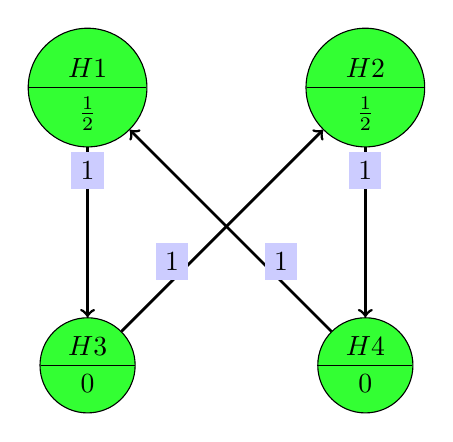
\begin{tikzpicture}[scale=1]
\node (H1) at (100bp,200bp) [draw,circle split,fill=green!80] {$H1$ \nodepart{lower} $\frac{1}{2}$};
\node (H2) at (200bp,200bp) [draw,circle split,fill=green!80] {$H2$ \nodepart{lower} $\frac{1}{2}$};
\node (H3) at (100bp,100bp) [draw,circle split,fill=green!80] {$H3$ \nodepart{lower} $0$};
\node (H4) at (200bp,100bp) [draw,circle split,fill=green!80] {$H4$ \nodepart{lower} $0$};
\draw [->,line width=1pt] (H1) to[auto] node[near start,above,fill=blue!20] {1} (H3);
\draw [->,line width=1pt] (H2) to[auto] node[near start,above,fill=blue!20] {1} (H4);
\draw [->,line width=1pt] (H3) to[auto] node[near start,above,fill=blue!20] {1} (H2);
\draw [->,line width=1pt] (H4) to[auto] node[near start,above,fill=blue!20] {1} (H1);
\end{tikzpicture}
  \caption{Graph corresponding to Examples 1 and 2 in \cite{Bretz11}}
\label{fig:bretz}
\end{figure}

\subsection{Creating Graphs using the gMCP GUI}
\label{sec:gMCPgui}

Alternatively one can specify graphs using the graphical user
interface provided by \gmcp.

\begin{knitrout}
\definecolor{shadecolor}{rgb}{0.969, 0.969, 0.969}\color{fgcolor}\begin{kframe}
\begin{alltt}
\hlkwd{library}\hlstd{(gMCP)}
\hlkwd{graphGUI}\hlstd{()}
\end{alltt}
\end{kframe}
\end{knitrout}


These commands will load the the \gmcp library and open the GUI
interface a screenshot of which is presented in Figure
\ref{fig:gui}. Graphs defined using this tool can be saved to an R
object the name of which can be specified in the line above the graph
manipulation window the graph is exported by setting the cursor into
this line (optionally editing the variable name) and pressing
enter. By default the variable name is set to createdGraph. This
creates an object of class \texttt{graphMCP}.

After switching back to R's interpreter the created graph can be
converted to a matrix using the command \texttt{graph2matrix} from
package \gmcp. The weights set for the graph can be extracted using
the function \texttt{getWeights}. 

\begin{knitrout}
\definecolor{shadecolor}{rgb}{0.969, 0.969, 0.969}\color{fgcolor}\begin{kframe}
\begin{alltt}
\hlstd{Gm} \hlkwb{<-} \hlkwd{graph2matrix}\hlstd{(createdGraph)}
\hlstd{w} \hlkwb{<-} \hlkwd{getWeights}\hlstd{(createdGraph)}
\end{alltt}
\end{kframe}
\end{knitrout}


Conversely graphs defined as matrices can also be converted to
\texttt{graphMCP} objects.

\begin{knitrout}
\definecolor{shadecolor}{rgb}{0.969, 0.969, 0.969}\color{fgcolor}\begin{kframe}
\begin{alltt}
\hlstd{G} \hlkwb{<-} \hlkwd{matrix2graph}\hlstd{(Gm,} \hlkwc{weights} \hlstd{= w)}
\hlkwd{graphGUI}\hlstd{(G)}
\end{alltt}
\end{kframe}
\end{knitrout}


\begin{figure}
  \centering
  \includegraphics[width=.95\textwidth]{pictures/example.png}
  
  \caption{Screenshot of \gmcp GUI }
\label{fig:gui}
\end{figure}


\section{Testing}
\label{sec:testing}

Performing tests using \gmcp can be done in several ways. \gmcp
provides functions covering every step in the test procedure which can
be done seperately or all together. The first step is the computation
of all intersection hypotheses in the closure of the test problem
together with conventional weights for the graphical approach without
knowledge of any correlations. This can be done using the function
\texttt{generateWeights}. For both of our examples this looks like:

\begin{knitrout}
\definecolor{shadecolor}{rgb}{0.969, 0.969, 0.969}\color{fgcolor}\begin{kframe}
\begin{alltt}
\hlkwd{library}\hlstd{(gMCP,} \hlkwc{quietly} \hlstd{=} \hlnum{TRUE}\hlstd{)}
\hlkwd{generateWeights}\hlstd{(Gm, w)}
\end{alltt}
\begin{verbatim}
##       [,1] [,2] [,3] [,4] [,5] [,6] [,7] [,8]
##  [1,]    0    0    0    1  0.0  0.0  0.0  1.0
##  [2,]    0    0    1    0  0.0  0.0  1.0  0.0
##  [3,]    0    0    1    1  0.0  0.0  0.5  0.5
##  [4,]    0    1    0    0  0.0  1.0  0.0  0.0
##  [5,]    0    1    0    1  0.0  1.0  0.0  0.0
##  [6,]    0    1    1    0  0.0  0.5  0.5  0.0
##  [7,]    0    1    1    1  0.0  0.5  0.5  0.0
##  [8,]    1    0    0    0  1.0  0.0  0.0  0.0
##  [9,]    1    0    0    1  0.5  0.0  0.0  0.5
## [10,]    1    0    1    0  1.0  0.0  0.0  0.0
## [11,]    1    0    1    1  0.5  0.0  0.0  0.5
## [12,]    1    1    0    0  0.5  0.5  0.0  0.0
## [13,]    1    1    0    1  0.5  0.5  0.0  0.0
## [14,]    1    1    1    0  0.5  0.5  0.0  0.0
## [15,]    1    1    1    1  0.5  0.5  0.0  0.0
\end{verbatim}
\end{kframe}
\end{knitrout}


\texttt{generateWeights} takes the graph defined as a matrix and the
vector of initial weights and returns a matrix where each row
corresponds to an intersection hypotheses in the closure of the test
problem. The first half of each line indicates the intersection
hypotheses. Hypotheses in the intersection are indicated by a $1$,
hypotheses not in the intersection are indicated by a $0$. For example
$(1,1,0,0)$ would stand for the intersection between $H_1$ and
$H_2$. The second half of the elements then provides weights for each
hypothesis in the corresponding intersection.

In a next step critical values for all elementary hypotheses in each
intersection hypothesis are computed. This can be done using
the function \texttt{generateBounds}. Here for the first time the
different assumptions on the correlation structure of Examples 1 and 2
are essential:

\begin{knitrout}
\definecolor{shadecolor}{rgb}{0.969, 0.969, 0.969}\color{fgcolor}\begin{kframe}
\begin{alltt}
\hlkwd{generateBounds}\hlstd{(Gm, w, Cm1,} \hlkwc{al} \hlstd{=} \hlnum{0.025}\hlstd{)}
\end{alltt}
\begin{verbatim}
##        [,1]  [,2]  [,3]  [,4]
##  [1,]    NA    NA    NA 1.960
##  [2,]    NA    NA 1.960    NA
##  [3,]    NA    NA 2.241 2.241
##  [4,]    NA 1.960    NA    NA
##  [5,]    NA 1.960    NA   Inf
##  [6,]    NA 2.241 2.241    NA
##  [7,]    NA 2.241 2.241   Inf
##  [8,] 1.960    NA    NA    NA
##  [9,] 2.241    NA    NA 2.241
## [10,] 1.960    NA   Inf    NA
## [11,] 2.241    NA   Inf 2.241
## [12,] 2.241 2.241    NA    NA
## [13,] 2.241 2.241    NA   Inf
## [14,] 2.241 2.241   Inf    NA
## [15,] 2.241 2.241   Inf   Inf
\end{verbatim}
\begin{alltt}
\hlkwd{generateBounds}\hlstd{(Gm, w, Cm2,} \hlkwc{al} \hlstd{=} \hlnum{0.025}\hlstd{)}
\end{alltt}
\begin{verbatim}
##        [,1]  [,2]  [,3]  [,4]
##  [1,]    NA    NA    NA 1.960
##  [2,]    NA    NA 1.960    NA
##  [3,]    NA    NA 2.212 2.212
##  [4,]    NA 1.960    NA    NA
##  [5,]    NA 1.960    NA   Inf
##  [6,]    NA 2.241 2.241    NA
##  [7,]    NA 2.241 2.241   Inf
##  [8,] 1.960    NA    NA    NA
##  [9,] 2.241    NA    NA 2.241
## [10,] 1.960    NA   Inf    NA
## [11,] 2.241    NA   Inf 2.241
## [12,] 2.212 2.212    NA    NA
## [13,] 2.212 2.212    NA   Inf
## [14,] 2.212 2.212   Inf    NA
## [15,] 2.212 2.212   Inf   Inf
\end{verbatim}
\end{kframe}
\end{knitrout}


Alternatively we could transform these error bounds into $p$-values to
recreate Table 2 of \cite{Bretz11}

\begin{knitrout}
\definecolor{shadecolor}{rgb}{0.969, 0.969, 0.969}\color{fgcolor}\begin{kframe}
\begin{alltt}
\hlstd{(}\hlnum{1} \hlopt{-} \hlkwd{pnorm}\hlstd{(}\hlkwd{generateBounds}\hlstd{(Gm, w, Cm2,} \hlkwc{al} \hlstd{=} \hlnum{0.025}\hlstd{)))} \hlopt{*} \hlnum{100}
\end{alltt}
\begin{verbatim}
##        [,1]  [,2]  [,3]  [,4]
##  [1,]    NA    NA    NA 2.500
##  [2,]    NA    NA 2.500    NA
##  [3,]    NA    NA 1.348 1.348
##  [4,]    NA 2.500    NA    NA
##  [5,]    NA 2.500    NA 0.000
##  [6,]    NA 1.250 1.250    NA
##  [7,]    NA 1.250 1.250 0.000
##  [8,] 2.500    NA    NA    NA
##  [9,] 1.250    NA    NA 1.250
## [10,] 2.500    NA 0.000    NA
## [11,] 1.250    NA 0.000 1.250
## [12,] 1.348 1.348    NA    NA
## [13,] 1.348 1.348    NA 0.000
## [14,] 1.348 1.348 0.000    NA
## [15,] 1.348 1.348 0.000 0.000
\end{verbatim}
\end{kframe}
\end{knitrout}


this function takes the graph in matrix form, the weights, the
correlation matrix and the overall \al as inputs in order to compute
rejection bounds for all elementary hypotheses in each intersection.
Bounds are computed using the multivariate distribution of test
statistics whenever the whole correlation matrix is known for more
than one test statistic associated with the elementary hypotheses
within the intersection. For a concise explanation of the involved
algorithm see \cite[Section 3.2]{Bretz11}.


Once rejection bounds have been computed overall rejection of
elementary hypotheses, based on actual data, needs to be determined
using the closed testing 
principle. This means that all hypotheses which are rejected in
all intersection hypotheses, of which they are a part of, are rejected
at the overall \al. 

Since the bounds of a testing procedure is independent of the
observed data \gmcp provides a test function for that particular
MTP: 

\begin{knitrout}
\definecolor{shadecolor}{rgb}{0.969, 0.969, 0.969}\color{fgcolor}\begin{kframe}
\begin{alltt}
\hlstd{Example1} \hlkwb{<-} \hlkwd{generateTest}\hlstd{(Gm, w, Cm1,} \hlkwc{al} \hlstd{=} \hlnum{0.025}\hlstd{)}
\hlstd{Example2} \hlkwb{<-} \hlkwd{generateTest}\hlstd{(Gm, w, Cm2,} \hlkwc{al} \hlstd{=} \hlnum{0.025}\hlstd{)}
\end{alltt}
\end{kframe}
\end{knitrout}


The definition of a test function is efficient if a test is applied
several times, for example in simulations.

The \texttt{myTest} function in the example above takes a vector of
three $z$-scores and returns results in the form of a boolean vector
wher \texttt{TRUE} stands for rejection of the null hypothesis and
\texttt{FALSE} signifies that the null has to be retained. 

\begin{knitrout}
\definecolor{shadecolor}{rgb}{0.969, 0.969, 0.969}\color{fgcolor}\begin{kframe}
\begin{alltt}
\hlkwd{Example1}\hlstd{(}\hlkwd{c}\hlstd{(}\hlnum{2.24}\hlstd{,} \hlnum{2.24}\hlstd{,} \hlnum{2.24}\hlstd{,} \hlnum{2.3}\hlstd{))}
\end{alltt}
\begin{verbatim}
## [1] FALSE FALSE FALSE FALSE
\end{verbatim}
\begin{alltt}
\hlkwd{Example2}\hlstd{(}\hlkwd{c}\hlstd{(}\hlnum{2.24}\hlstd{,} \hlnum{2.24}\hlstd{,} \hlnum{2.24}\hlstd{,} \hlnum{2.3}\hlstd{))}
\end{alltt}
\begin{verbatim}
## [1]  TRUE FALSE FALSE FALSE
\end{verbatim}
\end{kframe}
\end{knitrout}


We see that above $z$-score scenario leads to an effective gain in
power of the procedure when knowledge about the correlation structure
is used.

{\em Attention:} Not all scenarios of partial knowledge of the correlation
matrix can currently be handled by \gmcp. The correlation matrix must
have a block structure: We assume that the set of hypothesis can be
partitioned into subsets such that the pairwise correlations in each
subset are either known or are set to NA.  For
example assume that in the example given above not only correlations
between the statistics for $H_1$ and $H_2$ are known but also the
correlation between the statistics for $H_1$ and $H_3$ but not between
those associated with $H_2$ and $H_3$. In this case it is unclear when
testing the intersection hypotheses $H_1 \cap H_2 \cap H_3$ wether
the bounds for the statistics associated with $H_1$ and $H_2$ or
alternatively for those associated with $H_2$ and $H_3$ should
be searched using their multivariate distribution. The current
implementation would try to find bounds using the multivariate normal
distribution of all three statistics which is not fully known and
hence break and return an exception. 

\subsection{Testing using the gMCP interface}
\label{sec:gmcpint}

The function \gmcp provides a common interface to both sequentially
rejective Bonferroni procedures as well as parametric tests. \gmcp
takes objects of the type \texttt{graphMCP} as its input together with
a vector of $p$-values and computes whether the according test
procedure rejects. For Example 1 this amounts to the call:

\begin{knitrout}
\definecolor{shadecolor}{rgb}{0.969, 0.969, 0.969}\color{fgcolor}\begin{kframe}
\begin{alltt}
\hlstd{p} \hlkwb{<-} \hlnum{1} \hlopt{-} \hlkwd{pnorm}\hlstd{(}\hlkwd{c}\hlstd{(}\hlnum{2.24}\hlstd{,} \hlnum{2.24}\hlstd{,} \hlnum{2.24}\hlstd{,} \hlnum{2.3}\hlstd{))}
\hlstd{G} \hlkwb{<-} \hlkwd{matrix2graph}\hlstd{(Gm, w)}
\hlkwd{gMCP}\hlstd{(G, p)}
\end{alltt}
\begin{verbatim}
## gMCP-Result
## 
## Initial graph:
## A graphMCP graph
## H1 (weight=0.5)
## H2 (weight=0.5)
## H3 (weight=0)
## H4 (weight=0)
## Edges:
## H1  -( 1 )->  H3 
## H2  -( 1 )->  H4 
## H3  -( 1 )->  H2 
## H4  -( 1 )->  H1 
## 
## 
## P-values:
##      H1      H2      H3      H4 
## 0.01255 0.01255 0.01255 0.01072 
## 
## Adjusted p-values:
##      H1      H2      H3      H4 
## 0.02509 0.02509 0.02509 0.02509 
## 
## Alpha: 0.05 
## 
## Hypothesis rejected:
##   H1   H2   H3   H4 
## TRUE TRUE TRUE TRUE 
## 
## Final graph after 4 steps:
## A graphMCP graph
## H1 (rejected, weight=0)
## H2 (rejected, weight=0)
## H3 (rejected, weight=1)
## H4 (rejected, weight=0)
## No edges.
\end{verbatim}
\end{kframe}
\end{knitrout}


In the case of a sequentially rejective Bonferroni type procedure
\gmcp returns an object of class \texttt{graphMCP-Result} which holds
information on the specific sequence the test procedure has taken
through the graph and also provides adjusted $p$-values.

For Example 2 we use the same graph and assume normally distributed test
statistics with known variances and a correlation matrix of the form:

\begin{displaymath}
  \left( \begin{array}{cccc}
      1 & \frac{1}{2} & \texttt{NA} & \texttt{NA} \\
      \frac{1}{2} & 1 & \texttt{NA} & \texttt{NA} \\
      \texttt{NA} & \texttt{NA} & 1 & \frac{1}{2} \\
      \texttt{NA} & \texttt{NA} & \frac{1}{2} & 1
    \end{array} \right) .
\end{displaymath}

This can be implemented in \gmcp by additionally passing the correlation
matrix to \gmcp:

\begin{knitrout}
\definecolor{shadecolor}{rgb}{0.969, 0.969, 0.969}\color{fgcolor}\begin{kframe}
\begin{alltt}
\hlkwd{gMCP}\hlstd{(G, p,} \hlkwc{corr} \hlstd{= Cm2,} \hlkwc{test} \hlstd{=} \hlstr{"Bretz2011"}\hlstd{)}
\end{alltt}
\begin{verbatim}
## gMCP-Result
## 
## Initial graph:
## A graphMCP graph
## H1 (weight=0.5)
## H2 (weight=0.5)
## H3 (weight=0)
## H4 (weight=0)
## Edges:
## H1  -( 1 )->  H3 
## H2  -( 1 )->  H4 
## H3  -( 1 )->  H2 
## H4  -( 1 )->  H1 
## 
## 
## P-values:
##      H1      H2      H3      H4 
## 0.01255 0.01255 0.01255 0.01072 
## 
## Adjusted p-values:
##      H1      H2      H3      H4 
## 0.02332 0.02509 0.02509 0.02509 
## 
## Alpha: 0.05 
## 
## Hypothesis rejected:
##   H1   H2   H3   H4 
## TRUE TRUE TRUE TRUE
\end{verbatim}
\end{kframe}
\end{knitrout}


which returns a similar result however without the graphs representing
the rejection sequence, since the whole closed test is done in this
example. A vector specifying which of the elementary hypotheses
can be rejected at the overall \al. The reported $p$-values are the
unadjusted $p$-values passed to \gmcp. 

\newpage

\bibliography{literatur}

\end{document}
